\chapter{Host and Test Setup}
\label{chapter:host_and_Test_setup}

    To perform measurements and evaluate OpenStack, appropriate hardware is necessary.
    This hardware must also feature a certain OS, and the OpenStack components must be installed and configured.
    As embedded systems are not intended for Cloud Computing software like OpenStack, the installation and successful execution process includes difficulties.
    This chapter presents the hardware and software setup used for testing.
    
    
    \section{Hardware Setup}
    \label{section:hardware_setup}
        
        In order to study OpenStack on embedded systems, two different hardware platforms were chosen.
        To evaluate a broader spectrum of hardware, one platform was chosen to be x86-based, while the other was chosen to be an ARM-based platform.
        For the x86-based platform, an Intel Xeon Platinum \ac{CPU} with 24 cores was chosen.
        Due to having much computational power, systems based on this \ac{CPU} are currently used for developing autonomous driving.
        Therefore, this platform represents a powerful x86 embedded system intended for future use in automotive applications.
        The x86 platform comes further with 188 GB of memory and 960GB of NVMe secondary storage connected via a M.2 interface.\\
        A Renesas R-Car Starter Kit Pro, featuring a Renesas R-Car H3 SoC, was chosen for the ARM-based platform.
        With eight cores in a big.LITTLE architecture, this \ac{SoC} has four high-performance and four high-efficiency cores.
        It is specifically designed for the automotive industry and is currently used in automotive \acp{ECU}.
        The ARM platform comes with 4 GB of memory and a 64 GB SD-Card as secondary storage connected via an SD-Card interface.\\
        Table \ref{table:host_specs} shows the specifications of the hardware used.
        Both platforms are equipped with 1 Gbit network interfaces.
        The x86 platforms additionally come with a 10 Gbit network interface.

         \begin{table}[ht]
            \begin{center}
                \begin{tabular}{ c | c | c | c | c }
                    \textbf{Platform} 	& \textbf{Processor} 													& \textbf{Memory} 	& \textbf{Storage} 	& \textbf{Network} \\
                    \noalign{\hrule height 1.5pt}
                    x86			& \makecell[c]{Intel Xeon Platinum \\ 8160T @ 3.60 GHz (24 Cores)}				& 188 GB 			& 960 GB			& \makecell[c]{1x 1 Gbit \\ 1x 10 Gbit} \\[0.3cm]
                    ARM			& \makecell[c]{Renesas R-Car H3 \\ 4x Cortex-57 and 4x Cortex-53 } 			& 4 GB 			& 64 GB 			& 1x 1 Gbit
                \end{tabular}
            \caption{Hardware and specifications of the host systems used for testing}
            \label{table:host_specs}
            \end{center}        
        \end{table}
    
        \noindent Of each platform respectively, two systems were chosen to be used in the testing setup.
        As described in Section \ref{section:openstack}, an OpenStack cluster consists of different core services and additional separate components.
        Due to the high computational power and high memory, it was decided to configure one x86 platform as the controller node. 
        The other three nodes (2x ARM and 1x x86) were chosen to be configured as dedicated compute nodes.
        Figure \ref{figure:network_setup} shows the connection between all platforms, creating the OpenStack cluster.
        All platforms are connected via a Layer 2 1 Gbit Ethernet switch with Cat 5e Ethernet cables.
        However, the x86 platform configured as a compute node is in addition connected directly via a 10 Gbit Ethernet connection to the controller node.
        Further, the Ethernet switch is connected to a gateway via a 1 Gbit connection.
        The external network, though, is only used for installation and update purposes.
        
         \begin{figure}[ht]
             \begin{center} 
                    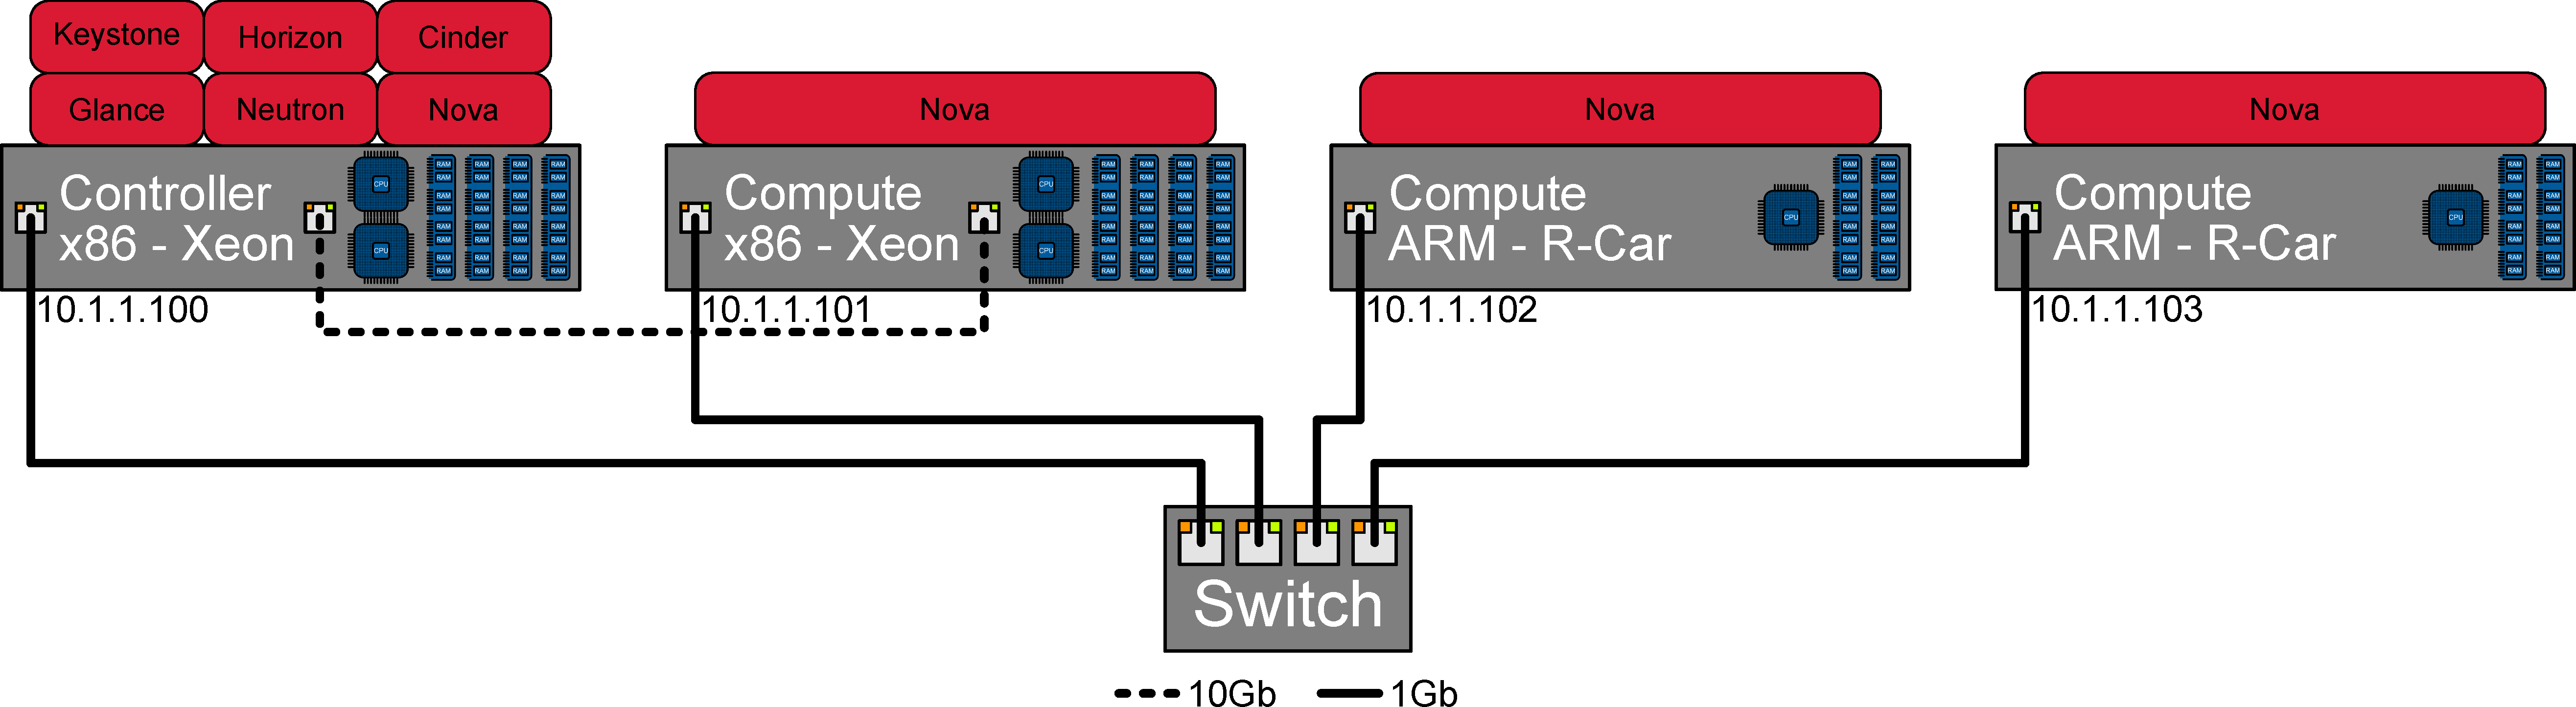
\includegraphics[width=\textwidth ]{03_network_setup.pdf} 
                    \caption{OpenStack hardware and network setup}
                    \label{figure:network_setup}
             \end{center}	
        \end{figure}
               
    
    \section{Software Installation}
    \label{section:software_installation}
        
        The installation process of all software consists of two stages.
        As a first step, the host system must be prepared.
        This preparation includes the OS, the correct configuration of necessary settings, and the installation of necessary packages and dependencies.
        As a second step, the OpenStack follows, including the installation and configuration of the OpenStack cluster.
        
        
        \subsection{Host System Preparation}
            
            Before installing the OpenStack services, the host systems must be prepared accordingly.
            For both platforms, Ubuntu 18.04 was chosen as the host \ac{OS} because of two reasons.
            First, Ubuntu is a Linux distribution supported and recommended by OpenStack, ensuring compatibility and better reliability with less unforeseeable complications.
            Second, using an Ubuntu distribution enables a simplified installation of OpenStack through DevStack\footnote{DevStack: https://docs.openstack.org/devstack/victoria/} and simplified interaction with the host system itself.
            For the x86 platform, an Ubuntu image already came prebuilt and preinstalled.
            Solely virtualization support had to be enabled in the BIOS settings.
            With the image being based on Ubuntu Server 18.04, a server \ac{OS} on primarily for server usage intended Intel Xeon \acp{CPU}, problems were neither anticipated nor encountered.
            
            \noindent Contrary to the Intel \acp{CPU}, the Renesas R-Car \acp{SoC} were neither intended to run Ubuntu as \ac{OS} nor OpenStack or similar software.
            This presents the first difficulty in integrating such \acp{SoC} as OpenStack nodes.
            The following paragraphs will briefly describe the problems and decisions made to prepare the \acp{SoC}.
            Table \ref{table:host_sw} shows the final \acp{OS} installed and the according kernel on each platform.
            
             \noindent \textbf{Installation of Ubuntu}
            Being an \ac{SoC} intended for embedded usage, the \ac{OS} usually is custom-built for the target system.
            Advantages of custom \acp{OS} lie in their small size by only including the necessary features, packages, and tools.
            To only include the necessary, all features and functionality in the form of packages must be known in advance.
            Together with a description of hardware features, a functional custom \ac{OS} can be created.
            As such image creation can be a tedious task, the Yocto Project was chosen for image creation.\\
            The Yocto Project\footnote{Yocto Project: https://www.yoctoproject.org} is an Open-Source project helping developers to create custom Linux-based systems \cite{Yocto2021}.
            Using the Yocto Project, packages needed in the image are specified through \textsl{recipes} and later \textsl{baked} into the final image.
            Similar, unique hardware properties are specified through the hardware manufacturer's board support packages and can be included in the image.\\
            Due to OpenStack's massive size, knowledge about all necessary packages and dependency in advance was impossible as this also includes all indirectly used libraries and packages.
            Although a particular repository exists, which aims at providing all recipes needed, tedious trials showed that the repository was not an option.
            Due to version constraints, the recipes for OpenStack were highly inconsistent, which hindered a successful image creation.\\
            For the final solution, it was decided to use a custom Yocto kernel along with a base version of Ubuntu.
            As Yocto generates all necessary outputs like kernel modules, they can be integrated and used by any \ac{OS}.
            To perform a successful installation of Ubuntu, the guide from \cite{Tnx942412020} was used and adapted accordingly.
            Summarized, both \acp{OS}, the Yocto generated and the Ubuntu one, were installed on separate partitions of an SD-Card.
            The Ubuntu OS was then configured to use the Yocto generated kernel and kernel modules.
            Although not having included the OpenStack packages into the image, the Ubuntu user space and especially aptitude enabled the standard way of installing any packages and other software.
            
             \noindent \textbf{Kernel Configuration}
            Using the described method to install Ubuntu relies on the kernel and the kernel modules built with the Yocto Project.
            As previously said, custom \acp{OS} contain only a minimal set of features and packages.
            The same applies to the kernel build with Yocto.
            Since OpenStack relies on many packages, which again rely on specific kernel modules, these kernel modules must be added explicitly to the kernel configuration in advance.
            By creating a kernel configuration file containing all necessary kernel modules and features, the Yocto build system can read which features and modules should be incorporated into the kernel.\\
            In addition to the basic Yocto kernel configuration, a few kernel modules have to be added.
            As OpenStack relies on network-based communication, \textsl{ebtables} and \textsl{netfilter} modules needed to be included.
            These modules enable the Linux firewall and packet filtering, which are substantial for OpenStack's internal communication.
            Further, \textsl{pseudo-filesystems} and \textsl{virtualization} had to be included.
            Pseudo-filesystems are necessary for OpenStack to keep track of the host systems' specific values and properties, while virtualization is necessary to virtualize resources.
            Last, the \textsl{device-mapper} module was necessary for OpenStack to manage storage as logical volumes for virtual machines.
            
             \noindent \textbf{Arm Trusted Firmware}
            As the last step in preparing the SoC the \ac{ATF} had to be reconfigured.
            The \ac{ATF} is a secure world software, that provides a trusted execution environment on a very low level \cite{Arm2021}.
            The crucial aspect of the \ac{ATF} for this thesis is that it must allow virtualization. 
            Otherwise, despite the kernel support, no virtualization of hardware resources is possible.
            In order to achieve this, individual files with specific configurations need to be generated. 
            Fortunately, Yocto also generates them automatically.
            Configuring the corresponding recipes to allow virtualization generates the according files.
            These files must then be flashed onto the \ac{SoC}.
            
            \begin{table}[ht]
            \centering
                    \begin{tabular}{ c | c | c }
                        \textbf{Platform} & \textbf{Kernel} 				& \textbf{OS} \\
                        \noalign{\hrule height 1.5pt}
                        x86			& 5.0.0-23-generic (x86\_64) 		& Ubuntu Server 18.04 \\
                        ARM			& 5.4.0-yocto-preempt-rt (aarch64)	& Ubuntu Base 18.04 
                    \end{tabular}
                \caption{Software specifications used on host systems for testing}
                \label{table:host_sw}   
            \end{table}
            
            
            
        \subsection{OpenStack Installation}
        \label{subsection:openstack_installation}
            
            Installing and configuring OpenStack can be a complicated, time-consuming, and error-prone task.
            Therefore, the DevStack scripts were chosen to install a complete OpenStack environment.
            OpenStack itself uses DevStack as a development environment and for functional testing.
            The future environment's configuration is made through a \textsl{local.conf} file, where parameters, settings, and services can be specified.
            In the following paragraphs, the configuration of the OpenStack cluster will be described and explained.
            
             \noindent \textbf{Installation}
            The DevStack documentation includes multiple different guides for installing an OpenStack environment.
            For the test scenarios and this thesis's scope, a multi-node environment was desired, with the main focus on compute services.
            Therefore, a minimal OpenStack configuration consisting of the services presented in Section \ref{subsection:components} was installed using the guide from \cite{OpenStackMNL2020}.
            Apart from Horizon, all services used represent the minimal set of services for an OpenStack environment.
            Horizon was also included for easier interaction with OpenStack and better visualization of current activities.
            As mentioned in Section \ref{section:hardware_setup}, an Intel Xeon node was chosen as the controller node due to its high computational power.
            All necessary core services were decided to be installed on this node, along with the compute services.
            This configuration makes the controller node also an all-in-one node.
            Evaluating the R-Car \acp{SoC} as a separate or additional controller node was not possible due to limited resources on the R-Car, especially the low memory.\\
            For the other nodes, only compute services and communication software was decided to be installed.
            The compute nodes were configured to communicate with the controller node if other services like network or storage services were needed.
            Due to later test purposes, a connection to the \acp{VM} was necessary, and the standard network configuration was not suitable.
            As OpenStack establishes a new internal network, there is no access from the external network possible.
            To make this possible, the OpenStack network's external interface needs to be connected to an actual physical interface.
            This can be achieved by specifying a public interface in the \textsl{local.conf} file, together with an exactly matching network configuration of the external network.
            Listings \ref{listing:local_conf_controller} and \ref{listing:local_conf_compute} show the final configuration files, which were used to install OpenStack.
                        
            \begin{listing}[htp]
                 \inputminted[frame=single, linenos, breaklines]{sh}{measurements/00_install-execute/03_local-conf-controller.sh}
                \caption{OpenStack controller node configuration file}
                \label{listing:local_conf_controller}
            \end{listing}
            
            \begin{listing}[htp]
                 \inputminted[frame=single, linenos, breaklines]{sh}{measurements/00_install-execute/03_local-conf-compute.sh}
                \caption{OpenStack compute node configuration file}
                \label{listing:local_conf_compute}
            \end{listing}

            \newpage
             \noindent \textbf{Post Installation Configuration}
            After installing OpenStack, all services were configured with default settings and standard configurations. 
            Although most of them were suitable and need not be changed, a few needed to be adjusted.
            The main configuration to adjust were the preconfigured flavors and images.
            DevStack automatically downloads and configures a Cirros x86 image for testing purposes.
            However, to mimic the host systems in the best way possible, Ubuntu 18.04 Cloud Images were chosen as guest images.
            Due to operating with two different \ac{CPU} architectures, one image for the x86 and one for the ARM-based platform was necessary.
            Both could be configured and uploaded to the Glance image service either via the command-line or the web interface.\\
            Next, DevStack also configures a couple of default flavors.
            A flavor in the context of OpenStack and overall Cloud Computing refers to the resource configuration of a \acp{VM}.
            Due to the intended testing of specific hardware in specific configurations, custom flavors had to be defined.
            Table \ref{table:flavors} lists all created and used flavors throughout this thesis.
            Distinct flavors were defined for each platform, as both platforms differ in performance capabilities.
            For each platform, one \textsl{max}-flavor was defined, representing the highest possible \ac{VM} configuration.
            The other flavors were derived from the minimal configuration on the ARM platform.
            Having to create \acp{VM} with at least one \ac{vCPU}, this corresponds to one-eighth of the host's \ac{CPU} resources on the ARM platform.
            Therefore, it was decided to create one flavor corresponding to one-eighth of all host's resources.
            The remaining flavors were derived by doubling the number of \acp{vCPU}, memory, and storage.\\
            Additional to the difference in \ac{CPU} architecture, the ARM platform further features a big.LITTLE architecture, consisting of four high-performance and four high-efficiency cores.
            At the time of writing this thesis, the KVM hypervisor cannot virtualize two different physical vCPUs simultaneously for one VM \cite{RussianNeuroMancer2019}.
            Trying to use high-efficiency and high-performance cores simultaneously results in an error of \ac{KVM}.
            To avoid \ac{KVM} choosing performance and efficiency cores simultaneously for one \ac{VM}, the flavors were configured to always and only use the performance cores.
            Therefore, the maximum number of virtualizable cores on the ARM hosts is reduced to four instead of eight.
             
            \noindent Finally, to access the \acp{VM} after creation, two additional settings needed to be changed.
            OpenStack, or rather Neutron, manages the traffic to the \acp{VM} using security rules.
            Based on these rules, only explicitly allowed traffic is forwarded from and to the \acp{VM}.
            In order to verify the connectivity of \acp{VM}, the internet control message protocol ICMP has to be allowed so that ping requests could reach the \acp{VM}.
            To further be able to log into the VM, \ac{SSH} connections had to be allowed.
            As Ubuntu Cloud Images disable password authentication via \ac{SSH} by default, authentication had to be performed using public and private key pairs.
            Ubuntu's Cloud Images use the cloud-init package\footnote{Cloud-Init Package: https://cloud-init.io} to retrieve additional information at the first boot from specific files or servers.
            OpenStack through Neutron provides a metadata service, which among others, can insert a specified public key into the \acp{VM} to enable a password-less \ac{SSH} authentication.
            
            \begin{table}[ht]
            \centering
                    \begin{tabular}{l !{\vrule width 1.5pt}  c | c | c | c | c}
                        \textbf{Name}	& \textbf{\makecell{rcar-01-\\256-06}}	&  \textbf{\makecell{rcar-02-\\256-06}	}	& \textbf{\makecell{rcar-01-\\512-06}}	& \textbf{\makecell{rcar-01-\\256-12}}	& \textbf{\makecell{rcar-max}}\\
                        \noalign{\hrule height 1.5pt}
                        \textbf{vCPUs}	& 1								& 2								& 1								& 1								& 4\\
                        \textbf{Memory}	& 256							& 256							& 512							& 256							& 2048\\
                        \textbf{Disk}	& 6								& 6								& 6								& 12								& 55\\
                        \multicolumn{1}{c}{}	& \multicolumn{1}{c}{}	& \multicolumn{1}{c}{}	& \multicolumn{1}{c}{}	& \multicolumn{1}{c}{}	& \multicolumn{1}{c}{}\\
                        \textbf{Name}	& \textbf{\makecell{xeon-06-\\21504-106}}	& \textbf{\makecell{xeon-12-\\21504-106}}	& \textbf{\makecell{xeon-06-\\43008-106}}	& \textbf{\makecell{xeon-06-\\21504-212}}	& \textbf{\makecell{xeon-max}}\\
                        \noalign{\hrule height 1.5pt}
                        \textbf{vCPUs}	& 6								& 12								& 6								& 6								& 48\\
                        \textbf{Memory}	& 21504							& 21504							& 43008							& 21504							& 174080\\
                        \textbf{Disk}	& 106							& 106							& 106							& 212							& 850\\
                    \end{tabular}
                \caption{OpenStack VM flavors}
                \label{table:flavors}
            \end{table}
            
            
            
            

            
            
            
    
    
    
    
    
    
    
    
    
    



